%%=============================================================================
%%  The ModelSEED Biochemistry Database: 2026 update
%%  Target journal: Nucleic Acids Research (NAR), Database Issue
%%  https://academic.oup.com/nar/pages/Ms_Prep_Database
%%
%%  This is the ONLY file that carries journal formatting. All prose lives in
%%  sections/ and is pulled in by the \input statements at the bottom.
%%  Build:  pdflatex main -> bibtex main -> pdflatex main -> pdflatex main
%%          (or simply: latexmk -pdf main.tex)
%%=============================================================================

%%-----------------------------------------------------------------------------
%%  NAR DATABASE-ISSUE REQUIREMENTS CHECKLIST
%%  Summary only. The authoritative, fully-cited version -- including OUP's
%%  figure format/dpi specification -- is in NAR_REQUIREMENTS.md alongside
%%  this file. Update that file, not this comment.
%%  (from academic.oup.com/nar/pages/Ms_Prep_Database, checked 2026-08-26)
%%
%%  [ ] LENGTH -- update papers: normally no more than 4-6 typeset journal
%%      pages. Contact the Executive Editor before submitting anything longer.
%%      Current draft is deliberately over; trim after [TBD] markers resolve.
%%  [!] TITLE -- the database name should ideally be the FIRST WORD of the
%%      title. Current title opens with "The". Consider "ModelSEED Biochemistry
%%      Database, 2026 update: ..." to comply.
%%  [ ] URL -- a working URL must appear BOTH in the abstract and in the body.
%%      See \modelseedurl below; used in the abstract. The body carries the
%%      repository URL in sections/data_availability.tex.
%%  [ ] GRAPHICAL ABSTRACT -- MANDATORY. 5:2 aspect ratio, min 127x50 mm
%%      (5x2 in), TIF/EPS/editable PDF, 300-600 dpi, landscape, sans-serif
%%      (Arial) 12-16 pt. Must be ORIGINAL -- not reused from any main or
%%      supplementary figure. No trademarked/copyrighted logos.
%%      Submitted as a separate file, not embedded here.
%%  [ ] REFERENCES -- numbered sequentially in order of appearance. The class
%%      default (no namedate/numbered option) gives NAR-style numeric (1,2).
%%      Exclude "submitted"/"in preparation"/personal communications.
%%      Cite other databases by their most recent published description; if
%%      none exists, put the URL in body text, NOT in the reference list.
%%  [ ] FIGURES -- no numeric limit on figure count; the 4-6 page budget is the
%%      real constraint. The database home page may NOT be used as a typeset
%%      figure. A representative screenshot of a query result IS allowed.
%%      Format (OUP artwork guidance): raster -> uncompressed .tif; vector ->
%%      .eps/.svg/.pdf with embedded fonts. Minimum dpi: 300 colour half-tone,
%%      600 greyscale, 600-900 combination/line art, 1200 mono line art; vector
%%      has no inherent resolution. RGB preferred. Arial/Times/Courier/Symbol,
%%      text >= 7pt, lines 0.25-1pt. Prefer vector PDF/EPS from the figure
%%      scripts -- it sidesteps the dpi table entirely. See NAR_REQUIREMENTS.md.
%%  [ ] DATA AVAILABILITY -- must address formats and terms for data download.
%%  [ ] DATABASE ACCESS -- must be freely accessible without login; HTTPS
%%      encouraged; URL persistence expected for >= 5 years post-publication.
%%      Mobile/tablet accessibility is worth mentioning explicitly.
%%  [ ] INITIAL SUBMISSION -- one .pdf with main text, references, tables and
%%      figures EMBEDDED. Supplementary data as separate file(s). Number all
%%      pages (the class does this). Single-column/single-spaced is waived for
%%      LaTeX, so the two-column class output is correct as-is.
%%      DO NOT use line-numbering. DO NOT use footnotes. (Verified absent.)
%%  [ ] DISCLOSURES -- ORCID REQUIRED for the submitting author. Author
%%      Contributions statement MANDATORY (CRediT encouraged). Conflict of
%%      interest disclosure REQUIRED. AI assistance used in preparing this
%%      manuscript MUST be disclosed in the cover letter and in Methods or
%%      Acknowledgements. See NAR_REQUIREMENTS.md section 13.
%%  [ ] CODE DEPOSIT -- a GitHub URL is not sufficient; deposit to Zenodo or
%%      FigShare and put the permanent DOI in Data Availability at revision.
%%  [ ] SUBMISSION -- at least six suggested referees (name, institute, email),
%%      independent, not same institution/city as any author. Handled in
%%      ScholarOne at submission time, not in this file.
%%  [ ] DEADLINE -- update manuscripts due 15 September. Nothing before 1 June.
%%-----------------------------------------------------------------------------

%% NAR specifies the OUP template's "Modern Large" design -- do not change these
%% two options without checking NAR_REQUIREMENTS.md section 7 first.
%% Modern/large gives: 9bp body on 11.5pt leading, SANS-SERIF body text
%% (modern is the only one of the three designs that forces \sffamily),
%% 7.5bp footnotes, 210x276mm paper, two columns.
%% Other designs exist (contemporary|traditional x large|medium|mediumone|small)
%% but are not what NAR asks for.
%% Omitting namedate/numbered keeps the class default = numeric citations (NAR style).
\documentclass[unnumsec,webpdf,modern,large]{oup-authoring-template}

%\onecolumn  % uncomment for a wide single-column reading/review draft

%%-----------------------------------------------------------------------------
%%  Packages. The class already loads: amsmath, amssymb, graphicx, hyperref,
%%  natbib, array, multirow, xcolor, tikz, url, caption, rotating, listings.
%%  It also defines \toprule / \midrule / \botrule itself -- do NOT load
%%  booktabs, it clashes.
%%-----------------------------------------------------------------------------
%% NOTE: the OUP manual asks authors to "refrain from adding further packages
%% or macros if possible", so nothing is loaded here. The draft-marker and
%% domain-shorthand macros below are the only additions, and the markers
%% disappear entirely under \draftmodefalse.

%%-----------------------------------------------------------------------------
%%  Draft markers.
%%  The source manuscript carries [TBD] and [DRAFT PENDING] placeholders.
%%  They are rendered in colour while drafting so they are impossible to miss.
%%  Flip \draftmodefalse (or pass \draftmodefalse before \begin{document})
%%  to make every marker vanish for a clean submission PDF.
%%-----------------------------------------------------------------------------
\newif\ifdraftmode
\draftmodetrue          % <-- set to \draftmodefalse for the submission build

\ifdraftmode
  \newcommand{\TBD}[1][]{\textcolor{red}{\textbf{[TBD}\ifx\relax#1\relax\else\ #1\fi\textbf{]}}}
  \newcommand{\DRAFTPENDING}[1]{\textcolor{orange}{\textbf{[DRAFT PENDING]}\ --\ #1}}
  \newcommand{\NUMBERSPENDING}[1]{\textcolor{orange}{\textbf{[NUMBERS PENDING]}\ #1}}
\else
  \newcommand{\TBD}[1][]{}
  \newcommand{\DRAFTPENDING}[1]{}
  \newcommand{\NUMBERSPENDING}[1]{}
\fi

%%-----------------------------------------------------------------------------
%%  Domain shorthands. Greek in text mode is unreliable under pdflatex, so all
%%  thermodynamic symbols route through math mode here.
%%-----------------------------------------------------------------------------
\newcommand{\dfG}{$\Delta_{\mathrm{f}}G'$}          % formation energy
\newcommand{\drG}{$\Delta_{\mathrm{r}}G'$}          % reaction energy
\newcommand{\drGo}{$\Delta_{\mathrm{r}}G'^{\circ}$} % standard reaction energy
\newcommand{\modelseedurl}{\url{https://modelseed.org}}
\newcommand{\repourl}{\url{https://github.com/ModelSEED/ModelSEEDDatabase}}
\newcommand{\file}[1]{\texttt{#1}}                  % repo paths / filenames
\newcommand{\cpd}[1]{\texttt{#1}}                   % compound identifiers

%% The OUP class sets \flushbottom (cls line 2513). With a short column the
%% slack is absorbed by the most elastic glue on the page -- the space above
%% \subsection headings -- which opened visible gaps before 'Atom mapping'
%% and 'Distribution and community process'. \raggedbottom lets a column end
%% short instead. Standard LaTeX, no package and no class option.
\raggedbottom

\begin{document}

%%-----------------------------------------------------------------------------
%%  Journal metadata -- production fills most of this in.
%%-----------------------------------------------------------------------------
%% The class calls \societylogo{} in the running head but leaves every
%% definition commented out (oup-authoring-template.cls:921-926), so it is
%% undefined unless the author supplies one. NAR is not a society journal with
%% a logo here, so the empty form the class itself offers is used. Without this
%% every build raised "Undefined control sequence" plus three "Missing number"
%% errors and still produced a PDF, which is why it went unnoticed.
\def\societylogo{}%
\journaltitle{Nucleic Acids Research}
\DOI{DOI added during production}
\copyrightyear{2026}
\pubyear{2026}
\vol{00}
\issue{0}
\access{Advance Access Publication Date: Day Month Year}
\appnotes{Database Issue}

\firstpage{1}
%% \lastpage must be set too. Unset, the class falls through \setlastpage to
%% its aux-file path, hands \relax to \@arabic and throws three "Missing
%% number, treated as zero" errors on every page shipout while still producing
%% a PDF. Update if the page count changes; production overwrites both.
\lastpage{6}

%\subtitle{Database Issue}

%%-----------------------------------------------------------------------------
%%  Title
%%  NAR: the database name should ideally be the first word. See checklist.
%%-----------------------------------------------------------------------------
%% Shortened 2026-09-15. The previous title's last clause -- "the impact of
%% reaction-direction assignments on metabolic-model output" -- promised an
%% analysis the paper does not contain: no section reports model output, flux
%% or biomass. Do not reinstate it without the analysis.
\title[ModelSEED Biochemistry Database, 2026 update]{The ModelSEED Biochemistry
Database, 2026 update: grading multi-source thermodynamics}

%%-----------------------------------------------------------------------------
%%  Authors
%%  \TBD -- the 2020 author list plus this cycle's contributors, minus anyone
%%  stepping off, in the agreed order. See PAPER_2026_PLAN.md open decision #3
%%  (untracked; local to the author's tree, not in the repository)
%%  for the Nikoloski-lab crediting format.
%%-----------------------------------------------------------------------------
%% ORCID is REQUIRED for the submitting author (NAR_REQUIREMENTS.md section 13).
%% Attach with \ORCID{0000-0000-0000-0000} directly after the author name.
%% AUTHOR LIST, per Sam 2026-09-07. Order: lead, then Argonne/Henry team with
%% the two interns, then the upstream-tool contributors grouped by tool, then
%% the KBase PIs, then the two corresponding authors last.
%%
%% SPELLINGS VERIFIED against published records, not transcribed. Five were
%% corrected from the names as first given:
%%   Beber      not "Bieber"    -- references.bib beber2022, and Seaver 2020
%%   Giessmann  not "Greissman" -- 10.3762/bjoc.19.26, IGDORE Berlin
%%   Setlur     not "Setler"    -- his fork, github.com/VibhavSetlur
%%   Wood-Charlson, Elisha M.   -- given only as "Elisha"; Seaver 2020
%%   Anand, Mohit               -- the third Maranas-lab author, 10.1371/journal.pcbi.1012516
%%                                 (novoStoic2.0, with Upadhyay and Maranas)
%% Faria, Edirisinghe, Liu, Arkin, Cottingham, Henry, Seaver all confirmed
%% against Seaver et al. 2020 (10.1093/nar/gkaa746).
%%
%% ORCIDs. Seven are CONFIRMED FROM A PUBLICATION -- the author list of
%% Seaver et al. 2020, read through Europe PMC's core result type, which
%% embeds ORCIDs per author:
%%   https://www.ebi.ac.uk/europepmc/webservices/rest/search?query=EXT_ID:32986834&resultType=core&format=json
%% Seaver's also cross-validates against the ORCID public API by name search,
%% which is the other reliable route:
%%   https://pub.orcid.org/v3.0/expanded-search/?q=family-name:X+AND+given-names:Y
%% Publisher pages are NOT a usable source: sciencedirect.com returns 403 to
%% automated fetches, as do AIP, RSC and ACS.
%%
%% Henry's ORCID 0000-0001-8058-9123 was confirmed by Chris himself
%% (2026-09-15), along with chenry@anl.gov. It is no longer inferred.
%%
%% STILL MISSING: Freiburger, Faria, Taylor, Setlur, Upadhyay, Anand, Maranas,
%% Giessmann, Wood-Charlson. Faria and Wood-Charlson carry no ORCID in either
%% paper checked, so those must come from the people themselves.
%%
%% AFFILIATION 9 (Penn State) is the only one still unconfirmed by the person
%% themselves. Noor (6), Beber (5) and Giessmann (3, 4) all supplied theirs
%% directly in Sept 2026. Numbering below runs in order of first appearance.
\author[1]{Andrew Freiburger\ORCID{0000-0002-7288-535X}}
\author[1]{Jos\'e P. Faria\ORCID{0000-0001-9302-7250}}
\author[1]{Janaka N. Edirisinghe\ORCID{0000-0003-2493-234X}}
\author[1]{Filipe Liu\ORCID{0000-0001-8701-2984}}
\author[2]{Cooper Taylor\ORCID{0009-0003-2147-1960}}
\author[1]{Vibhav Setlur\ORCID{0009-0000-6823-9761}}
\author[3,4]{Robert T. Giessmann}
\author[5]{Moritz E. Beber\ORCID{0000-0003-2406-1978}}
\author[6]{Elad Noor\ORCID{0000-0001-8776-4799}}
\author[7,8]{Vikas Upadhyay}
\author[9]{Mohit Anand}
\author[9]{Costas D. Maranas}
\author[10,11]{Sebastian Hu{\ss}\ORCID{0000-0003-0712-2986}}
\author[10,11]{Zoran Nikoloski\ORCID{0000-0003-2671-6763}}
\author[12]{Adam P. Arkin\ORCID{0000-0002-4999-2931}}
\author[13]{Robert W. Cottingham\ORCID{0000-0002-2775-3905}}
\author[12]{Elisha M. Wood-Charlson\ORCID{0000-0001-9557-7715}}
\author[1,$\dagger$]{Christopher S. Henry\ORCID{0000-0001-8058-9123}}
\author[1,$\ast$]{Samuel M. D. Seaver\ORCID{0000-0002-7674-5194}}

\address[1]{\orgdiv{Computing, Environment and Life Sciences Division},
\orgname{Argonne National Laboratory}, \orgaddress{\street{9700 S. Cass Ave.},
\postcode{60439}, \state{Lemont, IL}, \country{USA}}}

%% 2 supplied by Sam (2026-09-11) on Cooper Taylor moving from Argonne. No
%% postcode given, so none is written -- every other address here carries one.
\address[2]{\orgdiv{College of Engineering, Computing and Applied Sciences},
\orgname{Clemson University},
\orgaddress{\state{Clemson, SC}, \country{USA}}}

\address[3]{\orgname{Institute for Globally Distributed Open Research and Education (IGDORE)},
\orgaddress{\state{Berlin}, \country{Germany}}}

\address[4]{\orgdiv{Faculty II Mathematics and Natural Sciences, Institute of Chemistry, Chair of Biochemistry of Gas-Converting Biocatalysts},
\orgname{Technische Universit\"at Berlin},
\orgaddress{\state{Berlin}, \country{Germany}}}

\address[5]{\orgname{Institute for Globally Distributed Open Research and Education (IGDORE)},
\orgaddress{\state{Copenhagen}, \country{Denmark}}}

\address[6]{\orgdiv{Department of Plant and Environmental Sciences},
\orgname{Weizmann Institute of Science},
\orgaddress{\state{Rehovot}, \country{Israel}}}

%% 7 and 8 supplied by Vikas Upadhyay himself (2026-09-10) on moving from
%% Penn State; contact viku@illinois.edu. He holds both.
\address[7]{\orgdiv{NSF iBioFoundry},
\orgname{University of Illinois Urbana-Champaign},
\orgaddress{\postcode{61801}, \state{Urbana, IL}, \country{USA}}}

\address[8]{\orgdiv{Carl R. Woese Institute for Genomic Biology},
\orgname{University of Illinois Urbana-Champaign},
\orgaddress{\postcode{61801}, \state{Urbana, IL}, \country{USA}}}

\address[9]{\orgdiv{Department of Chemical Engineering},
\orgname{The Pennsylvania State University},
\orgaddress{\postcode{16802}, \state{University Park, PA}, \country{USA}}}

%% 10 and 11 are transcribed from Hu{\ss} et al. 2022 (10.1111/tpj.15903) via
%% Crossref, so they are 2022-vintage and unconfirmed by Hu{\ss} or Nikoloski:
%% confirm with them before submission.
\address[10]{\orgdiv{Systems Biology and Mathematical Modelling Group},
\orgname{Max Planck Institute of Molecular Plant Physiology},
\orgaddress{\street{Am M\"uhlenberg 1}, \postcode{14476}, \state{Potsdam},
\country{Germany}}}

\address[11]{\orgdiv{Bioinformatics, Institute of Biochemistry and Biology},
\orgname{University of Potsdam},
\orgaddress{\street{Karl-Liebknecht-Str. 24-25}, \postcode{14476},
\state{Potsdam}, \country{Germany}}}

\address[12]{\orgdiv{Environmental Genomics and Systems Biology Division},
\orgname{Lawrence Berkeley National Laboratory},
\orgaddress{\postcode{94720}, \state{Berkeley, CA}, \country{USA}}}

\address[13]{\orgdiv{Biosciences Division},
\orgname{Oak Ridge National Laboratory},
\orgaddress{\postcode{37830}, \state{Oak Ridge, TN}, \country{USA}}}

\corresp[$\ast$]{Corresponding author. \href{mailto:seaver@anl.gov}{seaver@anl.gov}}
\corresp[$\dagger$]{Corresponding author. \href{mailto:chenry@anl.gov}{chenry@anl.gov}}

%% Submission history. Left commented out deliberately: the month argument is
%% fed to \numexpr by the class (\myswitch, cls:1175), so an empty
%% \received{}{}{} throws "Missing number, treated as zero" -- once per macro --
%% while still producing a PDF. These dates are not knowable before submission
%% and are set by production. To use them, give a NUMERIC month:
%%   \received{1}{9}{2026}
%\received{}{}{}
%\revised{}{}{}
%\accepted{}{}{}

%%-----------------------------------------------------------------------------
%%  Abstract -- must contain a working URL (NAR requirement).
%%  Abstracts must stand alone: no citations to the reference list, no
%%  equations, no cross-references.
%%-----------------------------------------------------------------------------
\abstract{%% NAR: must contain a working URL; must stand alone (no citations, no
%% equations, no cross-references); keep as a SINGLE paragraph -- it is
%% \input into the \abstract{} argument in main.tex.
%%
%% Rewritten 2026-09-05 to the 6-page shape. Every number here is measured and
%% appears in the Results. Deliberately omitted, because the sections that
%% carried them are now Supplementary: PubChem validation, protein-carrier
%% cofactor standardisation, the reaction-similarity foundation model, and the
%% v2 draft-model direction-sensitivity study, which is not yet run.
The ModelSEED Biochemistry Database (\modelseedurl) supplies foundational mass- and charge-balanced reaction networks for metabolic reconstructions. Here we present an update on the biochemistry where the database has been expanded to $\sim46,000$ compounds, and $\sim56,000$ reactions, featuring $\sim37,000$ curated metabolic structures. We have expanded our approach for handling thermodynamic data, enabling multiple sources of data to be derived, integrated, and presented to the wider research community. We now publish predictions of pKa, reaction energy (and respective uncertainties) and estimates of reaction direction from multiple independent sources. We also provide an approach for grading the evidence classifying reactions at three different tiers: ``gold'', ``silver'', and ``bronze'', enabling users to transparently weigh reliability. We also provide predictions of reaction direction provided by an ensemble of LLMs. This multi-source approach exposes agreements and discrepancies between sources for $\sim33,000$ reactions. Finally, to ensure data integrity, a new conflict-resolution pipeline reconciles structures across sources, documenting input from curators. Our work is publicly available at \url{https://github.com/ModelSEED/ModelSEEDDatabase}.
}

\keywords{biochemistry database, metabolic modelling, thermodynamics,
atom mapping, reaction reversibility, ModelSEED}

\maketitle

%%=============================================================================
%%  BODY -- every section below is a separate file in sections/.
%%  Reorder, comment out, or add \input lines here; do not put prose in
%%  this file.
%%=============================================================================

\section{Introduction}

Hypotheses drawn and conclusions gained from the reconstruction, simulation, and analyses of metabolic reconstructions are only as good as the foundational biochemistry underpinning them. The ModelSEED Biochemistry Database was built to supply that layer: a mass- and charge-balanced reaction network, reconciled across the major biochemical databases~\cite{seaver2020}. Six years on, that layer is exercised mostly for integration: the 2020 release has been cited 193 times at an undiminished rate, and among citing papers with open full text 38\% use the database in their methods, overwhelmingly for genome-scale reconstruction. GEMsembler builds consensus models across tools, exploiting the fact that independent pipelines share the ModelSEED namespace to discard ambiguous identifier mappings~\cite{gemsembler2025} --- the ``Rosetta Stone'' function, exercised by someone other than us. Yeast9 assigned Gibbs energies to 98\% of its metabolites and 97\% of its reactions, taking from this database the metabolite values its other sources lacked~\cite{yeast9}.

This update reports the growth of the database, and an expanded approach in handling the layer of thermodynamics data allowing us to publish every source with its own uncertainty rather than promoting one. While over $70\%$ of the reactions with multiple sources of data agree on reaction direction, any disagreement is published for review by researchers to decide which numbers and approach carry weight.

Here we also describe a grading approach incorporating the uncertainities of the data across different sources, an integration of atom-mapping data to enable MFA analyses, and a structure-curation pipeline built to resolve conflict between structures from different databases. Finally, we expanded our search interface at https://modelseed.org for dissemination of the results.

\section{Materials and Methods}
%% Consolidates the former methods_{collation,integration,provenance,transport,
\subsection{Construction and Curation}\label{sec:methods-construction}

We collated additional compounds and reactions from MetaCyc~\cite{caspi2020}, Rhea~\cite{bansal2022}, and ChEBI~\cite{hastings2016}. The compounds are reconciled into single ModelSEED compounds using available structures where possible and the reactions are reconciled based on the identity of the compounds. The procedure follows the 2020 release~\cite{seaver2020}. Mass and charge balance is enforced and flagged.

For the 2020 release, a conflict between structures from multiple sources was either manually reviewed or dropped silently. The updated pipeline classifies each structural conflict and routes it to one of three outcomes: an automatic pick from the source variant matching the historical formula, a curator-authored override with recorded rationale, or an entry in a mass-balance exclusion registry for compounds where no source formula is defensible. Every outcome is attributed to its curator and its evidence. We retained every structure we collect, so conflict resolution can be inspected within the data in the repository. An outline of how a researcher can contribute is given in Supplementary Methods~S1 and expanded in the repository.
%% Rewritten 2026-09-08 after the Marvin 26.1 regeneration and the reversibility
%% overhaul. Every number here is measured against the shipped files; see the
%% inline comments for the command that reproduces each. Detail in
%% Supplementary Methods S2.
\subsection{Multi-source thermodynamics}\label{sec:methods-thermo}

The 2020 release combined two sources: the historical group contribution approach~\cite{jankowski2008} and eQuilibrator~\cite{flamholz2012}. This update carries four sources, each stored as its own record: group contribution, eQuilibrator~3.0~\cite{beber2022}, dGPredictor~\cite{wang2021}, and experimental values where they exist. Only the experimental values carry a published direction. The three predictors were released as energy estimators, so every direction reported here is an inference from their energies. All values are reported at pH~7.0, ionic strength 0.25\,M, pMg~3.0 and 298.15\,K; the basis for each condition and its effect on the released energies are given in Supplementary Methods~S2.

\paragraph{Protonation.} eQuilibrator's Legendre transform requires a \emph{macroscopic} pKa ladder per compound: an ordered list in which consecutive species differ by one proton. The count of entries around the desired pH sets the proton count of the major microspecies, so the composition of the ladder changes the transformed energy directly. We generate the pKa ladders using ChemAxon Marvin~\cite{marvin} for use with eQuilibrator, but we're conscious that these data cannot be regenerated without a license, so we also include the pKas generated by an open-source alternative, MolGpKa~\cite{pan2021}, for every compound with a structure, and the measured ladders of Alberty~\cite{alberty2003}, versioned per structure source in an extended pKa dictionary.

\paragraph{Experimental anchors.} eQuilibrator and dGPredictor both draw on the NIST Thermodynamics of Enzyme-catalyzed Reactions (TECR) Database~\cite{goldberg2004}, which is keyed to KEGG and reaches other namespaces through MetaNetX mappings that conflict structurally with ModelSEED identifiers. We therefore rebuilt the anchors, curating each conflict so that every TECR value maps directly onto a ModelSEED reaction, and evaluated openTECR (\url{https://github.com/opentecr}), a communal re-curation of the same source, to extend the set.

\paragraph{Uncertainty.} The three sources each adopt a different approach for estimating the uncertainty surrounding the predicted energy of reaction, so the scale of uncertainty is not directly comparable between them (Figure~\ref{fig:thermo}C). We therefore calibrate each source's reported uncertainty against the experimental anchors rather than reading it at face value; the resulting medians and the direction of each source's bias are reported with the results.

\paragraph{Direction.} For historical reasons, we use the same heuristics for deriving reaction direction from the Group contribution approach~\cite{jankowski2008} unchanged from 2020, so that series stays comparable across releases. For eQuilibrator and dGPredictor we use one rule set built on the reversibility index from Noor \textit{et al.}~\cite{noor2012}: a reaction is called irreversible when $|\ln\Gamma|$ exceeds $\ln(1000)$ by more than one propagated standard deviation~\cite{beber2022}, $\Gamma$ being the fold-change of reactant concentration required to change reaction direction). However, we extend the work by Noor \textit{et al.} to require the uncertainty to clear the threshold as well. We report fewer directions than the published index would on the same energies, and we separate \emph{reversible} reactions from \emph{undetermined} cases. An exception we implement is for reactions whose uncertainty is small relative to the threshold and yet still straddles it: meaning the estimate lies within one standard deviation of the threshold, and these we report as reversible.

\paragraph{Transport.} Compartments are \emph{relative} indices --- 0 inside, 1 outside --- not named compartments, so one reaction can be instantiated against a bacterial membrane, a mitochondrion or a plastid envelope when a template builds a model. Because the database is not committed to a cell type, transport reactions are scored from stoichiometry and energy alone: neither membrane potential nor pH gradient enters the estimate. The consequence is specific. A primary active transporter carries ATP hydrolysis in its stoichiometry, every predictor estimates that tightly, and the reaction earns a confident grade from chemistry that was never in question --- 96\% of gold-graded transport reactions are ATP-coupled and only 2.7\% translocate a proton. Such grades measure confidence in the coupled chemistry, not evidence that the transporter runs that way in a given organism; every reaction carries an \texttt{is\_transport} field so that this can be accounted for downstream. Reactions whose only change is of compartment carry no net chemistry and none is graded gold. dGPredictor commits on 1.4\% of transport reactions against 17.3\% elsewhere, so transport grades also rest on fewer independent sources.

%% Compact Methods statement for BOTH routes to a direction claim. The full
%% specification of each lives in the supplement:
%%   grading  -> Supplementary Methods S3
%%   ensemble -> Supplementary Methods S4
%% Do not re-expand either here; the budget is 4-6 typeset pages and the detail
%% was moved out deliberately.
\subsection{Grading reaction direction}\label{sec:methods-grading}

We apply a classification approach with which we grade the predicted reaction direction based on the available evidence. Very often sources and heuristics disagree, as is the case here, and we qualify what the reaction direction would be, and how reliable the evidence is using several tiers for ease of interpretation: gold, silver, or bronze. Our evaluation splits two ways, on the confidence of a source's own claim --- fitted as a probability against the experimental anchors --- and what the other sources make of it, by a weighted comparison on the same scale. Grades, self-assessments, and cross-source verdicts are stored in the biochemistry database, and can be viewed in the UI. The process of grading reactions is described fully in the Supplementary Methods.

\subsection{Ensemble LLMs predictions}\label{sec:llm-grading} Thermodynamic assignment is bounded by estimate coverage: energies cannot be computed for an incomplete reaction in terms of structures. Furthermore, every reaction is a member of a pathway within a cell, and the overarching drive of the pathway, dynamically changing metabolite concentrations as downstream enzymes process reagents, means a reaction may be driven in a direction on a level that supersedes our evaluation~\cite{mavrovouniotis1993,xu2008,noor2014}. We run a complementary approach using an ensemble, a ``council'' of large language models (LLMs) to interpret the reaction based on its name and stoichiometry alone. Three LLMs independently make their predictions, a fourth audits, and a fifth adjudicates. We list the prompts in the Supplementary Methods, along with the process and limits. We integrate these predictions transparently in our database, but do not include them in our grading of the thermodynamic evidence.
%% Consolidates the former methods_{reaction_similarity,atom_mapping} sections.
\subsection{Atom mapping}\label{sec:methods-mapping}

Atom mappings are generated from the workflow of Hu{\ss} \textit{et al.}~\cite{huss2022} where they refine the per-reaction output of the Reaction Decoder Tool~\cite{rahman2016} into mappings that can be used to span a metabolic reconstruction. The approach also resolves chemically equivalent atoms into symmetry groups --- such as the two oxygens of CO$_2$ and the six equivalent terminal oxygens of pyrophosphate --- so the ambiguity is apparent. The output is formatted and stored in the database, and can also be visualized in the UI.

\input{sections/M08_methods_distribution}

\section{Results}
%% Table 1 is the only table in the main text; the per-source breakdown that was
%% Table 3 in 2020 moves to Supplementary Table S1.
\subsection{Growth and coverage}\label{sec:results-growth}

The database has grown 34\% in compounds and 28\% in reactions since 2020, counting every record at both time points, driven mainly by MetaCyc and the BioCyc family. Reaction growth is now split across three primary databases (Figure~\ref{fig:growth}B): MetaCyc carries 31,805 reactions of which 21,258 are supplied by no other primary source, KEGG 14,066 of which 5,756 are unique, and the newly-integrated Rhea 17,477 of which 8,339 are unique: reactions the database would not otherwise hold. Completeness of reactions differs (Figure~\ref{fig:growth}C). We classify a complete reaction where every reagent can be assigned a complete molecular structure: 90\% of MetaCyc's and 76\% of KEGG's reactions against 66\% of Rhea's. Overall structure coverage rose from 28,120 to 36,943 compounds. The new biochemistry is not distributed like the old (Figure~\ref{fig:growth}D): the MetaCyc classes that grew are those of specialised metabolism --- antibiotic and polyketide biosynthesis, O-antigen and cell-envelope assembly, branched and acylated lipids, alkaloids --- while central carbon and energy metabolism account for 41 of the 12,261 reactions added. Central metabolism was already saturated in 2020; what a 2026 reconstruction gains is the periphery.
\subsection{Structure curation}\label{sec:results-structure}

We prioritised the curation pipeline on the compounds whose structures affect the ${\sim}9{,}000$ reactions carried by the ModelSEED and PlantSEED reconstruction templates, since an error in one of those propagates into every model built from them. The scope is a curation priority, not a statement about how much of the database is usable: the templates are discussed in Section~\ref{sec:results-mapping}. The conflict pipeline resolved every previously conflicting compound in three curation rounds. i) Instances where the conflict existed at the level of mobile hydrogens were resolved automatically using historical formula ii) instances where the structures were structurally different were resolved manually iii) instances where resolution was not straight-forward were entered in the mass-balance exclusion registry where we fix an arbitrarily chosen formula because no source formula was defensible.
\begin{figure*}[!t] \centerline{\includegraphics[width=\textwidth,page=2]{../figures/main_figures_draft.pdf}} \caption{\textbf{Thermodynamic sources.} (\textbf{A}) Provenance of every pK$_\mathrm{a}$ ladder shipped in the database, across all 45,708 compounds and 56,002 reactions. ChemAxon Marvin supplies 79.4\% of compounds and 81.6\% of reactions. \emph{Hatching} marks the share reached through a second route: the command-line calculator refuses polymers and organometallics as query molecules, so those are computed from SMILES through the Java plugin instead --- the same engine entered differently, agreeing to a median $|\Delta|$ of $0.0000$ over 300 compounds both routes accept. \emph{No ionizable site} is a result and not a gap --- Marvin reported no dissociable proton between pH $-2$ and $16$ for 1,242 compounds. The remainder carry no structure to compute from, which is a curation gap rather than a protonation one. (\textbf{B}) Reactions carrying a real energy from each source. (\textbf{C}) Reported uncertainty in kcal\,mol$^{-1}$, one axis per source because the three differ by more than an order of magnitude. The shaded band spans the 5th to 95th percentile, which is used in our classification scheme.} \label{fig:thermo} \end{figure*}

\subsection{Thermodynamics}\label{sec:results-thermo}

%% Counts measured 2026-09-08 from Biochemistry/reaction_*.json after the
%% Marvin 26.1 rebuild. Placeholders excluded per source: group contribution
%% dg = 1e7 (26,555 records); eQuilibrator sigma >= 2500 kcal/mol (3,386),
%% which is that source's refusal marker rather than an error bar.
The three predictors cover comparable fractions of the database and disagree substantially about how well they do it (Figure~\ref{fig:thermo}B). Uncertainty is reported on scales differing by more than an order of magnitude (Figure~\ref{fig:thermo}C): median 0.63\,kcal\,mol$^{-1}$ for eQuilibrator against 10.41 for group contribution and 17.01 for dGPredictor. 

\paragraph{Calibrating the reported errors against measurement.} That a source understates its error is measurable rather than asserted, and the experimental anchors are what measure it. For each source we collect one held-out prediction per anchored reaction --- a predicted energy and the uncertainty that source would report for it --- and divide the residual against the measured \drGo{} by that uncertainty. Measured this way, eQuilibrator's ratio has a root mean square of 8.06 and a median of 2.27, with only 28.7\% of reactions inside one standard deviation and 46.3\% inside two, indicating that eQuilibrator understates their error. Group contribution runs the other way, 73.6\% inside one standard deviation and a median ratio of 0.32 and dGPredictor is the best scaled of the three at 1.15 root mean square and 87.9\% inside one standard deviation. A researcher choosing by smallest reported error would systematically choose the source that understates it, which is the argument against promoting any single source. The grading in the next section calibrates each source's confidence against measurement rather than taking its uncertainty at face value.

\begin{figure*}[!t] \centerline{\includegraphics[width=\textwidth,page=3]{../figures/main_figures_draft.pdf}} \caption{\textbf{Direction, agreement and evidence.} (\textbf{A}) Direction assigned by each source independently: \emph{eQ} eQuilibrator, \emph{dG} dGPredictor, \emph{GC} group contribution, and \emph{LLMs} the large language model ensemble, which supplies a direction and no energy; its calls are released with the database and take no part in the evidence grading. Bar length is the number of reactions the source covers, so the rows are directly comparable. (\textbf{B}) What each evidence grade rests on by the deciding source's own calibrated confidence, and (\textbf{C}) by what the other sources made of it. The two panels share a scale but not a palette, so each carries its own key; categories are ranked as in Supplementary Table~1. \emph{Neither way} is the case that table writes \texttt{---}: a cross-check ran and settled neither way, so it neither helped nor penalised.} \label{fig:direction} \end{figure*}

\subsection{Direction assignment and evidence grading}\label{sec:results-direction}

%% All direction counts measured 2026-09-08 from Biochemistry/reaction_*.json
%% after the reversibility overhaul. Grades regenerated the same day against the
%% Marvin-26.1 energies with
%%   Scripts/Thermodynamics/SourceGrading/build_tecrdb_comparison.py
%%   Scripts/Thermodynamics/SourceGrading/grade_thermo_sources.py --cv
%% Anchors: 797 stereo-exact. The grade tiers are under active revision; the
%% rates below are for the scheme as it currently ships.
Each source now generates its own prediction for the direction each reaction proceeds, and the three sources differ more in what they will commit to than in what they say (Figure~\ref{fig:direction}A). eQuilibrator resolves 84.3\% of the reactions it covers, group contribution 42.9\% and dGPredictor 41.1\%. Across the database, 30,157 reactions receive a direction or a positive statement of reversibility from at least one source and 25,855 receive none.

\paragraph{eQuilibrator vs dGPredictor} dGPredictor is able to generate a predicted energy for more reactions ($\sim29,600$, against eQuilibrator's $\sim21,800$) and converts the least of that coverage into a usable reaction direction. For a typical dGPredictor reaction the error bar alone exceeds the decision threshold in the reversibility index, so 58.9\% of its reactions are returned undetermined against eQuilibrator's 15.7\%. Where both sources commit to a direction they agree 95.0\% of the time. dGPredictor is abstaining rather than contradicting, and it resolves 1,380 reactions eQuilibrator cannot, against 12,921 the other way.

\paragraph{Grading.} Of 33,099 graded reactions, 5,342 are gold, 16,498 silver and 11,259 bronze (Figure~\ref{fig:direction}D; see classification scheme in Supplementary Methods). The tiers separate on what supports them: gold is 85\% self-certain and 72\% corroborated, while bronze is 99\% unconfident and split between reactions no second source could check (48\%) and reactions the other sources contradict (35\%). Validated against the experimental anchors, gold reactions fall within 2\,kcal\,mol$^{-1}$ of measurement 94\% of the time ($n=439$) against 64\% at silver ($n=346$).

\paragraph{Recommendation.} Evidently where the sources agree on reaction direction, this becomes our recommendation, but because the sources can disagree, we prioritize the source from which we take the recommended reaction direction, so the priority order is eQuilibrator, dGPredictor, group contribution. eQuilibrator supplies 21,218 recommended reaction directions, dGPredictor 4,248 and group contribution 4,691; these numbers include the ones where there is agreement also. We record the source used to make the recommendation, so researchers may apply a different precedence.

%% Consolidates the former results_{atom_mapping,reaction_similarity,
%% connectivity_ontology} sections.
\subsection{Atom mapping}\label{sec:results-mapping}

Atom mappings are published for 26,242 reactions, 54\% of the database: 19,809 clean, and 6,433 that required salvage (which are tagged). As the mappings can be used to span a metabolic reconstruction, reactions needing one repair are likely to carry others.

\section{Discussion}

The change with the widest consequences here is a policy, not a number: no thermodynamic source is promoted over another. The 2020 release published one accepted value per reaction; this release publishes four, each with its own uncertainty and estimated direction, because the sources may disagree in ways a single value conceals. Grading against experiment enables us to validate the approach: A researcher can take the highest-graded source and knows what the grade means. In being explicit about disagreement between sources, we expect this release to serve the widening range of communities that build on shared biochemistry --- genome-scale reconstruction, flux analysis, pathway design and the training of predictive models.
\section{Data availability}

The ModelSEED Biochemistry Database is available at \url{https://github.com/ModelSEED/ModelSEEDDatabase} under the MIT licence, as versioned flat files and JSON. It is also queryable through a Solr endpoint and browsable at \modelseedurl. Released structures, thermodynamic values with per-source uncertainty, evidence grades, atom mappings and the low-confidence reaction flags are all in that repository. The scripts that regenerate every published value, including the eQuilibrator cache rebuild, are under \file{Scripts/Thermodynamics/}.

%% Supplied by Robert Giessmann (2026-09-14), his own wording. Only change:
%% ``wants to acknowledge'' -> ``acknowledges'' for journal register. NAR's
%% Article structure list places Acknowledgements before Author Contributions.
\section{Acknowledgements} R.T.G.\ acknowledges all the hard-working individuals who contributed their time voluntarily to transcribe and check the myriad of numbers and text to create the re-curated openTECR v1.0. The full list of contributors can be found at \url{https://github.com/opentecr}.

%% DRAFT for circulation, not agreed. Role assignment follows Sam's steer of
%% 2026-09-10: Sam lead throughout; Henry conceptualization plus funding and
%% supervision; Freiburger, Faria, Setlur and Taylor major, each supplying part
%% of the resources the release was assembled from; Edirisinghe and Liu minor.
%% External groups are credited for the tool or dataset they contributed.
%% Degrees (lead/equal/supporting) are CRediT's own qualifiers and carry the
%% major/minor distinction without ranking people. Every author must confirm
%% their own line: NAR requires editor approval to change roles after submission.
\section{Author contributions} Contributions follow the CRediT taxonomy. S.M.D.S.: conceptualization, methodology, software, formal analysis, data curation, visualization, writing -- original draft, project administration. C.S.H.: conceptualization, funding acquisition, supervision. A.F., J.P.F., V.S.\ and C.T.: resources, data curation, investigation; J.P.F.\ also writing -- original draft. J.N.E.\ and F.L.: resources, software (supporting). R.T.G.: the openTECR re-curation of the experimental measurements. E.N.\ and M.E.B.: eQuilibrator. V.U., M.A.\ and C.D.M.: dGPredictor. S.H.\ and Z.N.: atom mapping. A.P.A., R.W.C.\ and E.M.W.-C.: funding acquisition, supervision. All authors reviewed the manuscript.

\section{Funding}
%% Sam's wording, 2026-09-07. BRAVE's identifier is as he supplied it.
%%
%% KBase is cited with its FOUR EXTERNAL DOE AWARD NUMBERS, taken from the
%% funding acknowledgement of the most recent KBase paper. An earlier draft of
%% this section used PRJ1003559, which appears in cv.md and 19 times in the
%% mail archive -- but that is an INTERNAL Argonne cost code
%% ("PRJ1003559 66370 Kbase Pred Bio Environ"), not a DOE award number, and it
%% does not belong in a funding statement. Do not reinstate it.
%%
%% DE-AC02-06CH11357 deliberately appears TWICE: once as Argonne's operating
%% contract for this work, and once within KBase's own award list, where it is
%% Argonne's share of the KBase award. That is how KBase states it.
This work was supported by the U.S. Department of Energy, Office of Science, Biological and Environmental Research, under Argonne National Laboratory contract DE-AC02-06CH11357. We specifically acknowledge support from the BRAVE FWP (DOE-112-VAM-PRJ1011481). The DOE Systems Biology Knowledgebase (KBase) is funded by the U.S. Department of Energy, Office of Science, Office of Biological and Environmental Research, under Award Numbers DE-AC02-05CH11231, DE-AC02-06CH11357, DE-AC05-00OR22725, and DE-SC0012704.

\section{Conflict of interest} None declared.

\section{Notice of copyright} The submitted manuscript has been created by UChicago Argonne, LLC, Operator of Argonne National Laboratory (``Argonne''). Argonne, a U.S. Department of Energy Office of Science laboratory, is operated under Contract No.~DE-AC02-06CH11357. The U.S. Government retains for itself, and others acting on its behalf, a paid-up nonexclusive, irrevocable worldwide license in said article to reproduce, prepare derivative works, distribute copies to the public, and perform publicly and display publicly, by or on behalf of the Government. The Department of Energy will provide public access to these results of federally sponsored research in accordance with the DOE Public Access Plan. \url{http://energy.gov/downloads/doe-public-access-plan}


\bibliographystyle{oup-plain}
\bibliography{references}

\end{document}
